\documentclass[compress]{beamer}
\usepackage[utf8]{inputenc}
\usepackage[T1]{fontenc}
\usetheme{Singapore}
\usecolortheme{default}
\usepackage{graphicx}

\begin{document}
\title{Verschlüsselung mit GPG}  
\author{Sokü \& friends}
\date{} 

\frame{\titlepage} 

\frame{
  \frametitle{Struktur}
  \tableofcontents
} 

\section{Motivation}
\label{sec:motivation}

\begin{frame}
  \frametitle{Warum das alles eigentlich?}

  \begin{itemize}[<+(1)->]
  \item Emails können sehr leicht mitgelesen werden.
  \item Nur wer ein bisschen die Technik versteht, kann sich bewusst
    verhalten.
  \end{itemize}
\end{frame}

\section{Theorie}
\label{sec:theorie}
\begin{frame}
    \frametitle{\insertsection}
    \begin{description}
        \item[Verschlüsselung] Ich will nicht, dass alle wissen, was ich schreibe.
        \item[Authentifikation] Ich will mit der richtigen Person sprechen.
    \end{description}
\end{frame}

\subsection{Symmetrische und Asymmetrische Verschlüsselung}
\begin{frame}
  \frametitle{\insertsubsection}
  \begin{overprint}
    \onslide<1-4>
    \begin{description}
    \item[Symmetrische Verschlüsselung:] \alert{Ein} Schlüssel
      zum Verschlüsseln und wieder Entschlüsseln.
      
      \only<4>{Der Schlüssel muss
      sicher von der Senderin zum Empfänger gebracht werden. (alte
      Agentenfilme: Aktenkoffer mit Selbstzerstörung, das ist doch
      aufwändig)}
    \end{description}
    \onslide<5-7>
    \begin{description}
    \item[Asymmetrische Verschlüsselung:] Zwei
      Schlüssel: Ein \alert{öffentlicher} nur zum Verschlüsseln (darf
      auch den Bösen bekannt sein) und ein \alert{privater} zum
      Entschlüsseln (geheim, muss aber nicht mehr quer durch die Stadt
      getragen werden)
    \end{description}
    \onslide<8>
    \begin{description}
    \item[Wie geht das?] Mathe!  Zahlen multiplizieren geht leicht,
      Zahlen wieder aufteilen nicht.
    \end{description}
  \end{overprint}
  \vspace{1em}
  \begin{overlayarea}{\columnwidth}{8em}
    \includegraphics<2>[width=\columnwidth]{bilder/symmetric_schluessel.png}
    \includegraphics<3>[width=\columnwidth]{bilder/symmetric_text.png}
    \only<4>{
      \begin{center}
        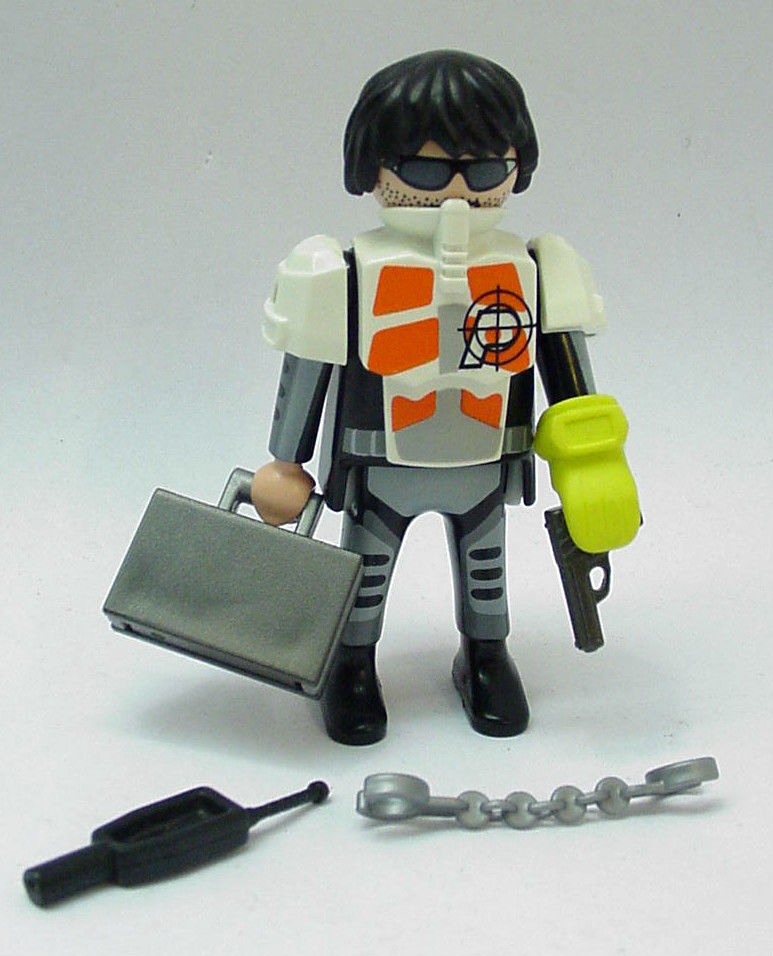
\includegraphics[height=9em]{bilder/agent_koffer.jpg}
      \end{center}
    }
    \includegraphics<6>[width=\columnwidth]{bilder/public_key_verfahren_schluessel.png}
    \includegraphics<7>[width=\columnwidth]{bilder/public_key_verfahren_text.png}
  \end{overlayarea}

\end{frame}

\subsection{Primzahlen rechnen}
\begin{frame}
  \frametitle{\insertsubsection}
  \begin{description}
  \item[Taschenrechner dabei?]
    \begin{itemize}
    \item 7 x 11 = ?
    \item 65 = ? x ? (5 x 13)
    \item 11251 x 2953 = 33224203
    \item 12883649 = ? (2957 x 4357) kann wohl niemand in unter einem
      Tag ausrechnen, auch mit Taschenrechner
    \end{itemize}
  \item[Verschlüsselung?] Das Produkt aus den zwei Primzahlen ist in
    etwa der öffentliche Schlüssel (auch die Geheimdienste können die
    Zahl nicht wieder aufspalten), die zwei kleinen Zahlen sind der
    private Schlüssel und müssen geheim bleiben.
  \end{description}
\end{frame}

\section{Theoretische Praxis}
\label{sec-1-1-4}

\begin{frame}
    \frametitle{Pretty Good Privacy}
    \onslide<2>
    Eine Methode asymmetrische Verschlüsselung umzusetzen ist
    \alert{P}retty \alert{G}ood \alert{P}rivacy, kurz PGP.
    \begin{itemize}
        \item benutzt Primzahlfaktorisierung
        \item stellt Signaturen bereit
    \end{itemize}
\end{frame}
\begin{frame}
    \frametitle{Schlüsselerstellung}
    \begin{description}
        \item[Theorie:] Generiere zufällige große Primzahlen
        \item[Praxis:] Maus bewegen
    \end{description}
\end{frame}
\begin{frame}
    \frametitle{Schlüsselaustausch}
    \begin{description}
        \item[Per Mail:] umständlich
        \item[Schlüsselserver:] Das schwarze Brett für PGP-Schlüssel
    \end{description}
    % Schlüsselaustausch und -server
\end{frame}
\begin{frame}
    \frametitle{Authentifikation}
    % Fingerprints und Signaturen
    Wem gehört der PGP-Schlüssel?
    \begin{description}
        \item[Signatur:] unterschreiben von Inhalten mit geheimen Schlüssel
        \item[Fingerprint:] Abbild vom öffentlichem Schlüssel
    \end{description}
    Signierte Mails reichen nicht, die Signatur muss auch stimmen!
    \onslide<2>
    \begin{itemize}
        \item Signieren von öffentlichen Schlüsseln möglich
        \item Überprüfen, ob die Mailadresse und öffentlicher Schlüssel zur Person passen
        \item Danach den Schlüssel signieren und auf Schlüsselserver laden
        \item Keysigning parties
    \end{itemize}
\end{frame}
\begin{frame}
    \frametitle{Widerrufen von Schlüsseln}
    Was tun wen's brennt?
    \begin{itemize}
        \item Passwort vergessen
        \item Private key verloren
        \item Rechner beschlagnahmt
    \end{itemize}
    Der Schlüssel darf nicht mehr verwendet werden!
    \onslide<2>
    \alert{Widerrufszertifikat} erklärt den Schlüssel für ungültig.

    Weiter: Ablaufdatum für Schlüssel
\end{frame}

\section{Die Praxis in der Theorie}
\label{sec-1-1-5}

\begin{frame}
  \frametitle{\insertsection}
  Programme zum Verschlüsseln:

  \begin{description}
  \item[gpg] \alert{G}nu\alert{P}rivacy\alert{G}uard, ein Programm zum
    Verschlüsseln und Signieren.  Heißt auf Windows \alert{GPG4Win}.
  \item[Enigmail] Ein Plugin für das Thunderbird-Mailprogramm, das gpg
    verwendet, um Mails zu verschlüsseln.
  \item[\ldots] Programme können auf anderen Systemen auch anders
    heißen.
  \end{description}

\end{frame}

\begin{frame}
  \frametitle{\insertsection{} -- Installation GPG4Win}
  Screenshots: Installation, Schlüsselgenerierung
  (Widerrufszertifikat!), Einrichtung Enigmail, Schlüssel hochladen,
  Schlüssel runterladen, Mail versenden, Mail empfangen
\end{frame}

\begin{frame}
  \frametitle{\insertsection{} -- Schlüsselgenerierung}
\end{frame}

\begin{frame}
  \frametitle{\insertsection{} -- Installation Enigmail}
\end{frame}

\begin{frame}
  \frametitle{\insertsection{} -- Enigmail einrichten}
\end{frame}

\begin{frame}
  \frametitle{\insertsection{} -- Schlüssel hochladen}
\end{frame}

\begin{frame}
  \frametitle{\insertsection{} -- Schlüssel runterladen}
\end{frame}

\begin{frame}
  \frametitle{\insertsection{} -- Mail versenden}
\end{frame}

\begin{frame}
  \frametitle{\insertsection{} -- Mail empfangen}
\end{frame}

\section{Praktische Praxis}
\label{sec-1-1-6}

\begin{frame}
  \frametitle{\insertsection}
  \begin{itemize}
  \item Runterladen/Verteilen
  \item Installieren
  \item \ldots{} (wie oben)
  \end{itemize}
  Vielleicht zuerst eine Mail an sich selber schreiben?
\end{frame}

\section{Weiterführendes}
\label{sec-1-1-7}

\begin{frame}
  \frametitle{\insertsection}
  \begin{itemize}
  \item Skript?
  \item Feedbackrunde
  \item Weitere Wünsche?
  \end{itemize}
\end{frame}
\end{document}
